\chapter{Edge detection}


\begin{description}
    \item[Edge] \marginnote{Edge}
        Pixel lying in between regions of the image with different intensities.
\end{description}



\section{Gradient thresholding}

\subsection{1D step-edge}
\marginnote{1D step-edge}

In the transition region, the absolute value of the first derivative grows (the absolute value is used as the polarity is not relevant).
By fixing a threshold, an edge can be detected.

\begin{figure}[H]
    \begin{subfigure}{0.4\linewidth}
        \centering
        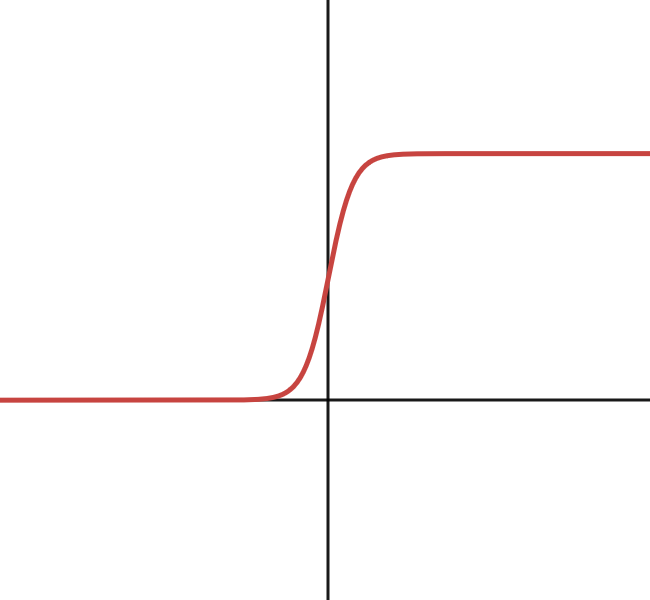
\includegraphics[width=0.5\linewidth]{./img/1d_step_edge_example1.png}
        \caption{Input signal}
    \end{subfigure}
    \begin{subfigure}{0.4\linewidth}
        \centering
        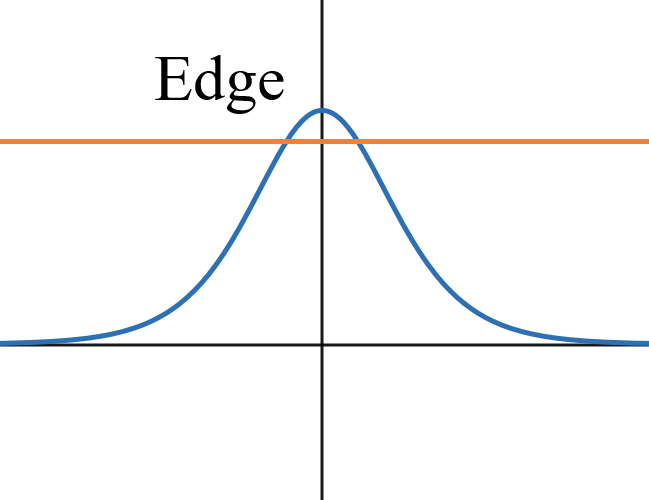
\includegraphics[width=0.5\linewidth]{./img/1d_step_edge_example2.png}
        \caption{Derivative of the signal}
    \end{subfigure}
\end{figure}


\subsection{2D step-edge}
\marginnote{2D step-edge}

In a 2D signal (e.g. an image), the gradient allows to determine the magnitude and the direction of the edge.
\[ 
    \nabla I(x, y) = 
    \begin{pmatrix} \frac{\partial I(x, y)}{\partial x} & \frac{\partial I(x, y)}{\partial y} \end{pmatrix} =
    \begin{pmatrix} \partial_x I & \partial_y I \end{pmatrix}
\]
\[
    \begin{split}
        \text{Magnitude: } & \Vert \nabla I(x, y) \Vert \\
        \text{Direction: } & \arctan\left(\frac{\partial_y I}{\partial_x I}\right) \in [-\frac{\pi}{2}, \frac{\pi}{2}] \\
        \text{Direction and sign: } & \arctan2(\partial_x I, \partial_y I) \in [0, 2\pi] \\
    \end{split}  
\]

\begin{description}
    \item[Discrete gradient approximation] \marginnote{Discrete gradient approximation}
        Approximation of the partial derivatives as a difference.
        \begin{description}
            \item[Backward difference] \marginnote{Backward difference}
                \[ \partial_x I(i, j) \approx I(i, j) - I(i, j-1) \hspace{3em} \partial_y I(i, j) \approx I(i, j) - I(i-1, j) \]


            \item[Forward difference] \marginnote{Forward difference}
                \[ \partial_x I(i, j) \approx I(i, j+1) - I(i, j) \hspace{3em} \partial_y I(i, j) \approx I(i+1, j) - I(i, j) \]

            \begin{remark}
                Forward and backward differences are equivalent to applying two cross-correlations with kernels 
                $\begin{pmatrix} -1 & 1 \end{pmatrix}$ and $\begin{pmatrix} -1 \\ 1 \end{pmatrix}$.
            \end{remark}

            \item[Central difference] \marginnote{Central difference}
                \[ \partial_x I(i, j) \approx I(i, j+1) - I(i, j-1) \hspace{3em} \partial_y I(i, j) \approx I(i+1, j) - I(i-1, j) \]
                
                \begin{remark}
                    Central difference is equivalent to applying two cross-correlations with kernels 
                    $\begin{pmatrix} -1 & 0 & 1 \end{pmatrix}$ and $\begin{pmatrix} -1 \\ 0 \\ 1 \end{pmatrix}$.
                \end{remark}
        \end{description}

    \item[Discete magnitude approximation] \marginnote{Discete magnitude approximation}
        The gradient magnitude can be approximated using the approximated partial derivatives:
        \[ 
            \Vert \nabla I \Vert = \sqrt{(\partial_x I)^2 + (\partial_y I)^2} \hspace{1.5em}
            \Vert \nabla I \Vert_+ = \vert \partial_x I \vert + \vert \partial_y I \vert \hspace{1.5em}
            \Vert \nabla I \Vert_\text{max} = \max(\vert \partial_x I \vert, \vert \partial_y I \vert)
        \]

        Among all, $\Vert \nabla I \Vert_\text{max}$ is the most isotropic (i.e. gives a more consistent response).
        \begin{example}
            Given the following images:
            \[
                E_v = \begin{pmatrix}
                    0 & 0 & h & h \\
                    0 & 0 & h & h \\
                    0 & 0 & h & h \\
                    0 & 0 & h & h \\
                \end{pmatrix}
                \,\,\,
                E_h = \begin{pmatrix}
                    0 & 0 & 0 & 0 \\
                    0 & 0 & 0 & 0 \\
                    h & h & h & h \\
                    h & h & h & h \\
                \end{pmatrix}
                \,\,\,
                E_d = \begin{pmatrix}
                    0 & 0 & 0 & 0 & h \\
                    0 & 0 & 0 & h & h \\
                    0 & 0 & h & h & h \\
                    0 & h & h & h & h \\
                \end{pmatrix}
            \]
            The magnitudes are:
            \begin{center}
                \begin{tabular}{c|ccc}
                    \toprule
                        & $\Vert \nabla I \Vert$ & $\Vert \nabla I \Vert_+$ & $\Vert \nabla I \Vert_\text{max}$ \\
                    \midrule
                    $E_h$ & $h$ & $h$ & $h$ \\
                    $E_v$ & $h$ & $h$ & $h$ \\
                    $E_d$ & $\sqrt{2}h$ & $2h$ & $h$ \\
                    \bottomrule
                \end{tabular}
            \end{center}
        \end{example}
\end{description}

\begin{remark}
    In practice, the signal of an image is not always smooth due to noise. 
    Derivatives amplify noise and are therefore unable to recognize edges.

    Smoothing the signal before computing the derivative allows to reduce the noise but also blurs the edges making it more difficult to localize them.

    A solution is to smooth and differentiate in a single operation by approximating the gradient as a difference of averages.
\end{remark}

\begin{description}
    \item[Smooth derivative] \marginnote{Smooth derivative}
        Compute the approximation of a partial derivative as the difference of the pixels in a given window.
        For instance, considering a window of 3 pixels, the cross-correlation kernels are:
        \[ \frac{1}{3} \begin{pmatrix} -1 & 1 \\ -1 & 1 \\ -1 & 1 \end{pmatrix} \hspace{3em} \frac{1}{3} \begin{pmatrix} -1 & -1 & -1 \\ 1 & 1 & 1 \end{pmatrix} \]

        \begin{description}
            \item[Prewitt operator] \marginnote{Prewitt operator}
                Derivative approximation using central differences.
                The cross-correlation kernels are:
                \[ 
                    \frac{1}{3} \begin{pmatrix} -1 & 0 & 1 \\ -1 & 0 & 1 \\ -1 & 0 & 1 \end{pmatrix} 
                    \hspace{3em} 
                    \frac{1}{3} \begin{pmatrix} -1 & -1 & -1 \\ 0 & 0 & 0 \\ 1 & 1 & 1 \end{pmatrix} 
                \]

            \item[Sobel operator] \marginnote{Sobel operator}
                Prewitt operator where the central pixels have a higher weight.
                The cross-correlation kernels are:
                \[ 
                    \frac{1}{4} \begin{pmatrix} -1 & 0 & 1 \\ -2 & 0 & 2 \\ -1 & 0 & 1 \end{pmatrix} 
                    \hspace{3em} 
                    \frac{1}{4} \begin{pmatrix} -1 & -2 & -1 \\ 0 & 0 & 0 \\ 1 & 2 & 1 \end{pmatrix} 
                \]
        \end{description}
\end{description}

\begin{remark}
    Thresholding is inaccurate as choosing the threshold is not straightforward.
    An image has strong and weak edges. Trying to detect one type might lead to poor detection of the other.

    A better solution is to find a local maxima of the absolute value of the derivatives.
\end{remark}



\section{Non-maxima suppression (NMS)}
\marginnote{Non-maxima suppression (NMS)}

Algorithm that looks for local maxima of the absolute value of the gradient along the gradient direction.

The algorithm works as follows:
\begin{enumerate}
    \item Given a pixel at coordinates $(i, j)$,
        estimate the magnitude $G = \Vert \nabla I(i, j) \Vert$ and the direction $\theta$ of the gradient.
    \item Consider two points $A$ and $B$ along the direction $\theta$ passing through $(i, j)$
        and compute their gradient magnitudes $G_A$ and $G_B$.
    \item Substitute the pixel $(i, j)$ as follows:
        \[ \texttt{NMS}(i, j) = \begin{cases}
            1 & (G > G_A) \land (G > G_B) \text{ (i.e. local maximum)} \\
            0 & \text{otherwise} \\
        \end{cases} \]
\end{enumerate}

\begin{remark}
    After applying NMS, the resulting signal (now composed of 0s and 1s) is converted back to the original gradient magnitudes
    in such a way that pixels 0ed by NMS remain 0 and pixels set at 1 by NMS return to their original value.

    After the conversion, a thresholding step might be applied to filter out unwanted edges that are either due to noise or not relevant.
\end{remark}


\subsection{Linear interpolation}

As there might not be two points $A$, $B$ along the direction $\theta$ belonging the the discrete pixel grid,
it is possible to use linear interpolation to estimate the gradient of these points even if off-grid of an offset $\Delta x$:\\
\begin{minipage}{0.6\linewidth}
    \[
        \begin{split}
            G_1 &= \Vert \nabla I(i-1, j) \Vert \hspace{2em} G_2 = \Vert \nabla I(i-1, j+1) \Vert \\
            G_3 &= \Vert \nabla I(i+1, j) \Vert \hspace{2em} G_4 = \Vert \nabla I(i+1, j-1) \Vert \\
        \end{split}
    \]
    \[
        \begin{split}
            G_A &\approx G1 + (G2 - G1)\Delta x \\
            G_B &\approx G3 - (G3 - G4)\Delta x \\
        \end{split}
    \]
\end{minipage}
\begin{minipage}{0.35\linewidth}
    \centering
    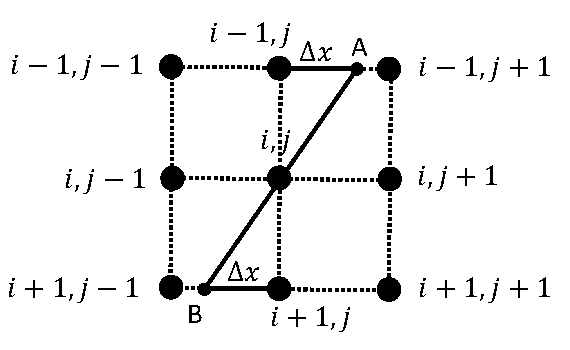
\includegraphics[width=\linewidth]{./img/_nms_interpolation.pdf}
\end{minipage}